\section{Pi} \label{sec:pi}

I dette afsnit beskrives det overordnede design på den software der kommer til at ligge på Pi. På figur \ref{fig:cd_pi} ses et klassediagram der opdeler funktionaliteten i klasser.

\begin{figure}[h]
\centering
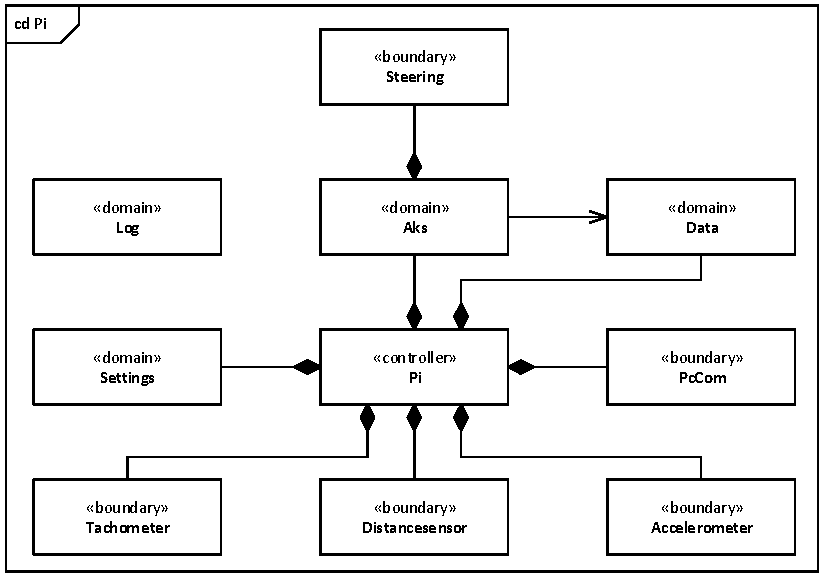
\includegraphics[width=\textwidth* 9/10]{../fig/diagrammer/bil/cd_pi.pdf}
\caption{Klasse diagram over Pi}
\label{fig:cd_pi}
\end{figure}

\subsection{Controller-klasse: Pi}
Controller-klassen Pi indeholder main funktionen og har derfor ansvaret for at styre slagets gang. Klassen skal derfor iværksætte initialisering af alle de klasser som den har ejerskab over. En af klassen ansvarsområder er at indsamle data fra sensorerne, og dette gøres ved at starte en særskilt tråd til dette. Denne tråd skal også sørge for at iværksætte Aks-klassen hver gang nye data er indsamlet.

\subsection{Domain-klasse: Aks}
Domain-klassen analyserer indkomne sensordata og i tilfælde at bilen er ved at køre ind i en forhindring, blokeres brugerinput og der styres udenom eller bremses.

\subsection{Domain-klasse: Data}
Denne klasse har til formål at indsamle alle sensordata i en datastruktur. Disse data gemmes i memory kan ikke overstige en defineret størrelse. Brugerinput gemmes ikke i denne klasse.

\subsection{Domain-klasse: Log}
Denne klasse har til formål at gemme samtlige systemhændelser i den fil, så kilden til eventuelle programcrash kan identificeres. Alle klasser på Pi har en reference til denne log, så de hver i sær kan skrive til den. På figur \ref{fig:cd_pi} er der undladt at lave pile fra alle klasser til denne, da dette vil gøre diagrammet uoverskueligt. 

\subsection{Domain-klasse: Settings}
Settings er datastruktur der indeholder indstillinger for maksimal hastighed, AKS status, og styretøjs kalibrering. Indstillingerne er gemt i en fil som kan tilgås af Pi-klassen og Steering-klassen.

\subsection{Boundary-klasse: PcCom}
Boundary-klassen PcCom håndterer kommunikationen imellem PC og Bil. Denne kommunikation sker vha. UDP via Wi-Fi.

\subsection{Boundary-klasse: Steering}
I denne klasse styres bilens aktautorer. Dette er altså en driver til både motoren der skaber fremdrift og servo-motoren der styrer forhjulene. Klassen tager ligeledes højde for brugers indstillinger.

\subsection{Boundary-klasse: Tachometer}
Denne klasse håndterer kommunikationen til bilens tachometer og konverterer sensordata til brugbar hastighedsmåling.

\subsection{Boundary-klasse: Distancesensor}
Denne klasse håndterer kommunikationen til bilens afstandssensorer og konverterer sensordata til brugbar distancemålinger. Klasen håndterer alle fire sensorer.

\subsection{Boundary-klasse: Accelerometer}
Denne klasse håndterer kommunikationen til bilens accelerometer og konverterer sensordata til brugbar g-måling.